Questo capitolo è una rapida presentazione di alcuni concetti di geoemtria differenziale: più nello specifico di geometria Riemanniana, con prevalente riferimento a \cite[Part~II]{milnor1963morse} e \cite[Capitoli~6-7]{abate2011geometria}.

Sia \(M\) una varietà differenziabile liscia di dimensione \(n\). Nel seguito, con \textit{liscia} si intende \(C^\infty\). Inoltre assumiamo sempre che \(M\) sia connessa e senza bordo. Denotiamo:
\begin{itemize}[label=]
	\item \(C^\infty(M)\) lo spazio delle funzioni \(f:M \to \R\) lisce;
	\item \(T_pM\) lo spazio tangente a \(M\) in \(p\);
	\item \(\pi: TM \to M\) il fibrato tangente;
	\item \(\T(M)\) lo spazio dei campi vettoriali lisci su \(M\).
\end{itemize}

\begin{defi}
	Una varietà compatta e senza bordo si dice \textit{chiusa}. 
\end{defi}

\section{Connessioni e derivate covarianti}
	
	Una \textit{connessione} su una varietà è un modo di derivare un campo vettoriale lungo una qualunque direzione in maniera ‘‘chiusa'', cioè in modo tale che il risultato sia un vettore tangente. Quanto segue è tratto principalmente da \cite[Chapter~8]{milnor1963morse} e \cite[Sezione~6.1]{abate2011geometria}.
	
	\begin{defi}
		Una \textit{connessione affine} su un punto \(p \in M\) è una mappa bilineare
		\begin{align*}
			\nabla^p:T_pM \times \T(M) &\to T_pM \\
			(X_p,Y) &\mapsto \nabla^p_{X_p}Y = \nabla_{X_p}Y
		\end{align*}
		che soddisfi
		\[
		\nabla_{X_p} fY = (X_pf) Y + f(p)\nabla_{X_p}Y 
		\]
		per ogni \(X_p \in T_pM, \ f \in C^\infty(M), \ Y \in \T(M)\). Il vettore \(\nabla_{X_p}Y\) è detto \textit{derivata covariante} di \(Y\) lungo \(X_p\).
		
		Una \textit{connessione affine globale} (o in breve \textit{connessione}) su \(M\) è una mappa che associa a ogni \(p \in M\) una connessione affine \(\nabla^p\) su \(p\) tale che l'applicazione
		\begin{align*}
			\nabla: \T(M) \times \T(M) &\to \T(M)\\
			(X,Y) &\mapsto \nabla_X Y,
		\end{align*}
		definita da \((\nabla_XY)_p \coloneq \nabla^p_{X_p}Y\), sia ben definita, cioè \(\nabla_X Y \in \T(M)\).
	\end{defi}
	\begin{oss}
		Una connessione su \(M\) soddisfa le seguenti proprietà:
		\begin{enumerate}[label=(\roman*)]
			\item \(\nabla:\T(M) \times \T(M) \to \T(M)\) è bilineare;
			\item \(\nabla_{fX}Y = f \nabla_XY\) per ogni \(f \in C^\infty(M)\), \(X,Y \in \T(M)\);
			\item \(\nabla_X(fY)= (Xf)Y+f\nabla_XY\) per ogni \(f \in C^\infty(M)\), \(X,Y \in \T(M)\).
		\end{enumerate}
		
		Se \((u^1,\dots , u^n)\) sono coordinate su un aperto \(U \subset M\), una connessione \(\nabla\) su \(U\) è univocamente determinata da \(n^3\) funzioni \(\Gamma_{ij}^k\), dette \textit{simboli di Christoffel}. Infatti, sia \(\de_k = \de/\de u^k \in \T(U)\) il frame della carta e scriviamo ogni campo \(X \in \T(U)\) come
		\[
		X= \sum_k  x^k \de_k
		\]
		per delle funzioni \(x^k \in C^\infty(U)\). In particolare, per ogni \(i,j\),
		\[
		\nabla_{\de_i} \de_j = \sum_k \Gamma_{ij}^k\de_k
		\]
		e quindi, usando le proprietà di connessione, per ogni \(X,Y \in \T(U)\) si ottiene che
		\begin{equation*}
			\nabla_X Y = \sum_{k}\left(Xy^k+\sum_{i,j}\Gamma_{ij}^kx^iy^j\right) \de_k.
		\end{equation*}
		
		Inoltre, date \(n^3\) funzioni \(\Gamma^k_{ij}\), questa formula definisce una connessione su \(U\). Per i dettagli, si può vedere \cite[Osservazione~6.1.9]{abate2011geometria}
	\end{oss}
	
	\begin{es}[Connessione piatta]\label{es: connessione patta}
		In \(\R^n\) possiamo definire la connessione data dalla derivata direzionale in ogni componente
		\[
			\nabla_ X Y \coloneq \sum_k (Xy^k) \de_k
		\]
		cioè con tutti i simboli di Christoffel nulli. Questa connessione è detta \textit{connessione piatta}. 
	\end{es}

	\begin{defi}\label{def: curva}
		Una \textit{curva parametrizzata} (o semplicemente \textit{curva}) è una mappa liscia \(\gamma: J \to M\), con \(J\) una varietà (differenziabile) 1-dimensionale, quindi \(J=\R\) (o un intervallo aperto) oppure \(J=\Sp^1 = \R/\Z\).  Talvolta prenderemo \(J=[a,b]\), intendendo che \(\gamma\) è la restrizione di una curva definita su un intervallo aperto che contiene \([a,b]\). Se \(J= \Sp^1\), diremo che \(\gamma\) è una \textit{curva chiusa}. 
	\end{defi}
	Una curva chiusa \(\gamma:\Sp^1 \to M\) si solleva in modo unico a una curva definita su \(\R\), denotata ancora \(\gamma:\R \to M\), che è 1-periodica, ovvero \(\gamma(t)=\gamma(t+1)\) per ogni \(t \in \R\).
	
	\begin{defi}
		Un \textit{campo vettoriale lungo una curva} \(\gamma:J \to M\) è una funzione
		\begin{align*}
			V: J &\to TM \\
			t &\mapsto V_t
		\end{align*}
		tale che \(V_t \in T_{\gamma(t)}M\) e che \(Vf \in C^\infty(J)\) per ogni \(f \in C^\infty(M)\), dove \(Vf(t):=V_t f\) per ogni \(t \in J\). Lo spazio vettoriale dei campi lungo \(\gamma\) è denotato \(\T(\gamma)\). 
		
		Il campo vettoriale \textit{velocità} (o \textit{vettore tangente}) di una curva \(\gamma:\R \to M\) è 
		\[
		\dot \gamma = \frac{\dif \gamma}{\dif t} \coloneq \dif \gamma \frac{\dif}{\dif t} \in \T(\gamma)
		\]
		dove
		\[
		\dif \gamma:T\R \to TM
		\]
		è il differenziale di \(\gamma\) e \(\dif/\dif t\) è il campo vettoriale standard di \(\R\). Se \(\gamma\) è chiusa, allora la velocità della curva solevata è 1-periodica, e quindi passa al quoziente, definendo la velocità della curva \(\dot \gamma:\Sp^1 \to TM\) sulla circonferenza \(\Sp^1\). 
	\end{defi}
	
	\begin{lemma}
		Sia \(\nabla\) una connessione su \(M\) e \(\gamma:\R \to M\) una curva. Allora esiste un unico operatore lineare
		\begin{align*}
			D_\gamma: \T(\gamma) \to \T(\gamma)
		\end{align*}
		tale che
		\begin{enumerate}[label=(\roman*)]
			\item per ogni \(f \in C^\infty(\R)\) e \(V \in \T(\gamma)\),
			\[
			D_\gamma (fV) =\dot f V + fD_\gamma V;
			\]
			dove \(\dot f = \dif f / \dif t\);
			\item se \(V \in \T(\gamma)\) è indotto da \(\widetilde{V} \in \T(M)\), cioè 
			\[
			V_t = \widetilde{V}_{\gamma(t)} \qquad \forall t \in \R,
			\]
			allora
			\[
			\left(D_\gamma V\right)_t = \nabla_{\dot{\gamma}(t)}\widetilde{V} \qquad \forall t \in \R.
			\]
		\end{enumerate}
	\end{lemma}
	\begin{proof} L'unicità segue dalla (ii), che in coordinate dà la formula 
		\begin{equation*}
			D_\gamma V = \sum_k \left(\dot v^k + \sum_{i,j}(\Gamma_{ij}^k \circ \gamma) \dot u^i v^j \right) (\de_k)_{\gamma}.
		\end{equation*}
		per \(V = \sum_k v^k (\de_k)_\gamma\). L'esistenza si ottiene definendo \(D_\gamma\) con tale formula. Per i dettagli si può vedere \cite[Lemma~8.1]{milnor1963morse} oppure \cite[Proposizione~6.1.12]{abate2011geometria}
	\end{proof}
	
	\begin{defi}
		L'operatore \(D_\gamma\) è detto \textit{derivata covariante lungo} \(\gamma\). 
	\end{defi}
	
	\begin{defi}
		Una connessione \(\nabla\) su \(M\) è detta \textit{simmetrica} se per ogni \(X,Y \in \T(M)\)
		\[
		\nabla_X Y - \nabla_YX = [X,Y],
		\]
		dove \([X,Y]\) denota le \textit{Lie-brackets} di \(X\) e \(Y\), definite da
		\[
		[X,Y] f \coloneq X(Yf) - Y(Xf) \qquad \forall f \in C^\infty(M).
		\]
	\end{defi}
	\begin{oss}
		Sia \(\nabla\) una connessione su \(M\). In coordinate, siccome \([\de_i,\de_j]=0\), se \(\nabla\) è simmetrica allora
		\[
		\Gamma_{ij}^k= \Gamma_{ji}^k.
		\]
		Viceversa, se \(\Gamma_{ij}^k = \Gamma_{ji}^k\) per ogni scelta di coordinate, si verifica facilente che \(\nabla\) è simmetrica.
	\end{oss}
	\begin{es}
		La connessione piatta definita nell'Esempio~\ref{es: connessione patta} è simmetrica. 
	\end{es}
	
	
	
	\section{Varietà Riemanniane}
	
	La geometria Riemanniana studia le varietà differenziabili in cui è possibile misurare lunghezza e angoli, e di conseguenza in cui è possibile quantificare la nozione di curvatura. Tuttavia la nozione di curvatura va oltre lo scopo del capitolo, pertanto in questa sezione viene data solo la definizione di metrica Riemanniana e connessione di Levi-Civita, seguendo soprattutto \cite[Chapter~8]{milnor1963morse} e \cite[Sezioni~6.5-6]{abate2011geometria}.
	
	\begin{defi}
		Una \textit{metrica Riemanniana} su una varietà \(M\) è una mappa \(g\) che a ogni punto \(p \in M\) associa un prodotto scalare \(g_p : T_p M \times T_pM \to \R\) e tale che, per ogni scelta di coordinate \((u^1,\dots, u^n)\) su \(U\subset M\), le funzioni
		\begin{align*}
			g_{ij}:U &\to \R \\
			p &\mapsto g_p((\de_i)_p,(\de_j)_p)
		\end{align*}
		siano \(C^\infty\). La coppia \((M,g)\) è detta \textit{varietà Riemanniana}. Talvolta denoteremo \(g_p = \langle \cdot,\cdot \rangle_p\) e \(| \cdot |_p\) la norma su \(T_pM\) indotta da \(g_p\). 
	\end{defi}
	
	\begin{es}[Metrica piatta]\label{es: metrica piatta}
		In \(\R^n\) il prodotto scalare standard induce una metrica Riemanniana, detta \textit{metrica piatta}. I coefficienti metrici sono
		\[
			g_{ij} \equiv \delta_{ij} = \begin{cases}
				1 & \text{ se } i = j \\
				0 & \text{ se } i \neq j
			\end{cases}
		\]
	\end{es}
	
	\begin{lemma}\label{lemma: frame ortonormale}
		Per ogni \(p \in M\) esiste un frame ortonormale locale, cioè esiste un intorno \(U\) e dei campi \(E_1,\dots,E_n \in \T(U)\) tali che in ogni punto di \(U\) formino una base ortonormale dello spazio tangente. 
	\end{lemma}
	\begin{proof}
		È sufficiente prendere una carta locale che contenga \(p\) e applicare il procedimento di ortonormalizzazione di Gram-Schmidt al frame \(\de_1, \dots,\de_n\). 
	\end{proof}
	
	Grazie alla metrica Riemanniana, è possibile definire la lunghezza di una curva. Diremo che una mappa continua \(\gamma:[a,b] \to M\) è una curva \textit{curva liscia regolare a tratti} se esiste una partizione \(a=t_0<t_1< \dots < t_k=b\) di \([a,b]\) tale che per ogni \(i \in \{1,\dots, k\}\) la restrizione \(\gamma|_{[t_{i-1},t_i]}\) sia una curva liscia (cf. Definizione~\ref{def: curva}) con vettore tangente sempre non nullo. Denotiamo con \(C^\infty_{piec}([a,b],M)\) l'insieme di tali curve. La \textit{lunghezza} di una curva \(\gamma \in C^\infty_{piec}([a,b],M)\) è 
	\begin{equation}\label{eq: funzionale lunghezza}
	L(\gamma) \coloneq \int_a^b |\dot \gamma(t) |_{\gamma(t)} \ \dif t. 
	\end{equation}
	
	È naturale dunque porre su \(M\) la seguente distanza: per ogni \(p,q \in M\)
	\[
	d(p,q) \coloneq \inf\{L(\gamma) \ | \ \gamma \in C^\infty_{piec}([0,1],M) \text{ t.c. } \gamma(0)= p, \gamma(1)=q\}.
	\]
	È immediato verificare che \(d\) è una distanza su \(M\). Seguirà dalla Proposizione~\ref{prop: proprietà locali exp} che \(d\) induce su \(M\) la stessa topologia che induce la struttura di varietà.
		
	%%distanza indotta dalla metrica

\begin{figure}[h]
	\centering
	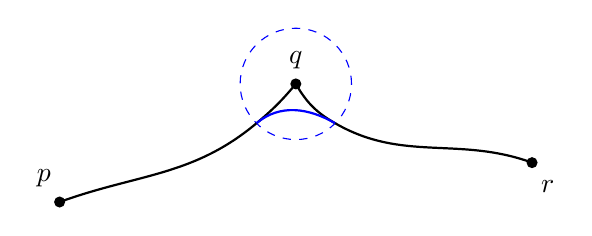
\begin{tikzpicture}
		%\draw [help lines] (-4,-2) grid (4,2);
		\fill (-3,-1)circle (2pt);
		\node at (-3.2,-0.7){\(p\)};
		\fill (0,.5) circle (2pt);
		\node at (0,0.8){\(q\)};
		\fill (3,-0.5) circle (2pt);
		\node at (3.2,-0.8){\(r\)};
		\draw[blue, dashed] (0,.5) circle (0.7071);
		\draw[thick] (-3,-1) to[out=20,in=220](-.5,0) to[out=40, in =230](0,.5) to[out=300, in=150] (.5,0) to[out=330, in=160] (3,-0.5);
		\draw[thick, blue] (-.5,0) to[out=40, in=150] (.5,0);

		
	\end{tikzpicture}
	
	\caption{Costruzione per dimostrare la disuguaglianza triangolare}
	
	\label{fig: metrica}
	
\end{figure}
	
	
	Data una curva \(\gamma: \R \to M\) regolare, cioè tale che \(\dot \gamma(t) \neq 0\) per ogni \(t \in \R\), la metrica Riemanniana permette sempre di riparametrizzare in maniera naturale la curva con la \textit{lunghezza d'arco}:
	\[
		s(t) \coloneq \int_0^t |\dot \gamma(u)| \ \dif u, \qquad t \in \R
	\]
	è un diffeomorfismo perché \(\dot s = |\dot \gamma| \neq 0\). La curva \(\gamma \circ s^{-1}\) è la \textit{riparametrizzazione in lunghezza d'arco} di \(\gamma\). Notare che \(\gamma\)  è parametrizzata in lunghezza d'arco, cioè \(s = \id\), se e solo se \(|\dot \gamma | \equiv 1\).
	
	
	Passiamo allo studio della relazione tra metrica Riemanniana e connessione. Rendiamo precisa la nozione di compatibilità tra queste due strutture.
	\begin{defi}
		Una connessione \(\nabla\) su \(M\) si dice \textit{compatibile} con la metrica \(g\) se per ogni curva \(\gamma:\R \to M\) e per ogni coppia di campi \(V,W \in \T(\gamma)\) vale 
		\[
		\frac{\dif}{\dif t} \langle V,W\rangle_\gamma = \left\langle D_\gamma V, W \right\rangle_\gamma + \left\langle V, D_\gamma W \right\rangle_\gamma.
		\]
	\end{defi}

	\begin{teo}[Levi-Civita]
		Ogni varietà Riemanniana \((M,g)\) ammette un'unica connessione simmetrica \(\nabla\) compatibile con la metrica \(g\), detta connessione di Levi-Civita. Inoltre in ogni carta i simboli di Christoffel sono dati da
		\begin{equation}\label{eq: simboli Christoffel di Levi-Civita}
		\Gamma_{ij}^k = \frac{1}{2} \sum_l g^{kl}\left( \frac{\de g_{lj}}{\de u^i} + \frac{\de g_{il}}{\de u^j} - \frac{\de g_{ij}}{\de u^l} \right),
		\end{equation}
		dove \((g^{ij})\) è la matrice inversa di \((g_{ij})\)
	\end{teo}
	\begin{proof}
		L'unicità si ottiene derivando le funzioni \(g_{ij} = g(\de_i,\de_j)\) per ottenere la formula (\ref{eq: simboli Christoffel di Levi-Civita}) in ogni carta. L'esistenza si mostra verificando che i simboli di Christoffel definiti da (\ref{eq: simboli Christoffel di Levi-Civita}) danno una connessione compatibile con la metrica Riemanniana. Per i dettagli si veda \cite[Teorema~6.6.6]{abate2011geometria} oppure \cite[Lemma~8.6]{milnor1963morse}.
	\end{proof}
	\begin{es}
		La connessione di Levi Civita della metrica piatta è la connessione piatta.
	\end{es}

	
\section{Sottovarietà Riemanniane}\label{sez: sottovarietà}
	
	Con l'intento di rendere più semplice il problema dal punto di vista variazionale, nei prossimi capitoli adotteremo spesso un approccio estrinseco, cioè considereremo delle sottovarietà \(M \subset \R^N\): è dunque necessario definire cos'è una sottovarietà Riemanniana ed esaminarne alcune proprietà. Questa sezione è tratta principalmente da \cite[Section~8.1]{lee1997riemannian}. Ricordiamo le seguenti definizioni.
	\begin{defi}
		Siano \(M\) e \(N\) due varietà differenziabili. Una mappa liscia \(j:M \to N\) si dice un \textit{embedding} se \(j\) è un omeomorfismo con l'immagine e per ogni \(p \in M\) il differenziale \(dj_p:T_pM \to T_{j(p)}N\) è iniettivo.
	\end{defi}
	
	\begin{defi}
		Una varietà differenziabile \(S\) si dice una \textit{sottovarietà differenziabile} di \(M\) se \(S \subset M\) e l'inclusione \(i:S \hookrightarrow M\) è un embedding. 
	\end{defi} 
	
	\begin{defi}
		Siano \(M\) una varietà differenziabile, \((N,g)\) una varietà Riemanniana e \(j:M \to N\) un embedding. La \textit{metrica pull-back} su \(M\) è la metrica \(j^*g\) definita da
		\[
		(j^*g)_p(v,w) \coloneq g_{j(p)}(\dif j_pv,\dif j_p w)
		\]
		per ogni \(p \in M\) e \(v,w \in T_pM\). 
	\end{defi}
	Non è difficile verificare che \(j^*g\) sia effettivamente una metrica Riemanniana su \(M\).
	
	\begin{defi}
		Una \textit{sottovarietà Riemanniana} \(M \subset \widetilde{M}\) della varietà Riemanniana \((\widetilde{M},\widetilde{g})\) è una sottovarietà differenziabile dotata della metrica pull-back \(g=i^*\widetilde{g}\) (denotata anche \(\widetilde{g}|_S\)), dove \(i:M \to \widetilde{M}\) è l'inclusione. La varietà \(\widetilde{M}\) è detta \textit{varietà ambiente} e la metrica \(g\) è anche detta \textit{metrica indotta} da \(\widetilde{g}\) su \(M\). 
	\end{defi}
	
	\begin{defi}
		Un embedding \(j:(M,g^M) \to (N,g^N)\) tra varietà Riemanniane si dice \textit{isometrico} se \(g^M = j^*g^N\).
	\end{defi}
	
	Un risultato (profondo) di J. Nash \cite{nash1956imbedding} garantisce che ogni varietà Riemanniana può essere vista come una sottovarietà di \(\R^N\), dotato della metrica piatta, per \(N\) sufficientemente grande.
	
	\begin{teo}[Nash]\label{teo: embedding isometrico di Nash}
		Ogni varietà Riemanniana ammette un embedding isometrico in \(\R^N\), considerato con la metrica piatta. 
	\end{teo}
	Per una dimostrazione si veda \cite[Theorem 3.1.1]{delellis2017masterpieces}.
	
	Sia \((\widetilde{M},\widetilde{g})\) una varietà Riemanniana di dimensione \(N\) e consideriamo una sottovarietà \((M,g)\) di dimensione \(n\). Tutti i simboli tildati si riferiscono a \(\widetilde{M}\), altrimenti sono le restrizioni a \(M\). Siccome \(g\) e \(\widetilde{g}\) coincidono quando sono definiti entrambi, possiamo denotarle entrambe con \(\langle\cdot ,\cdot\rangle\) senza rischio di confusione. 
	
	In maniera naturale, l'insieme
	\[
	T\widetilde{M}|_M \coloneq \coprod_{p \in M} T_p\widetilde{M}
	\]
	è un fibrato vettoriale di rango \(N\) su \(M\) e una sottovarietà di \(T \widetilde{M}\), detto \textit{fibrato tangente ambiente} su \(M\). Inoltre ogni sezione liscia di \(T\widetilde{M}\) si restringe a una sezione liscia di \(T\widetilde{M}|_M\) e viceversa ogni sezione liscia di \(T\widetilde{M}|_M\) si può estendere a una sezione liscia di \(T\widetilde{M}\) (si veda \cite[p. 132]{lee1997riemannian}). Denoteremo con \(\T(\widetilde{M}|_M)\) lo spazio delle sezioni lisce di \(T\widetilde{M}|_M\).
	
	In ogni punto \(p \in M\), lo spazio tangente ambiente \(T_p\widetilde{M}\) si decompone in somma diretta, ovvero
	\[
	T_p\widetilde{M} = T_pM \oplus N_pM
	\]
	dove \(N_pM \coloneq (T_pM)^\perp\) è lo \textit{spazio normale} a \(p\) rispetto a \(\widetilde{g}_p\) su \(T_p\widetilde{M}\). L'insieme
	\[
	NM \coloneq \coprod_{p \in M}N_pM
	\]
	è naturalmente un fibrato vettoriale di rango \(N-n\) su \(M\) e una sottovarietà di \(T\widetilde{M}|_M\), detto \textit{fibrato normale} di \(M\) (si veda \cite[p. 133]{lee1997riemannian}). Denoteremo con \(\mathcal{N}(M)\) lo spazio delle sezioni lisce di \(NM\).
	
	La proiezione ortogonale a ogni punto \(p\) di \(T_p\widetilde{M}\) su \(T_pM\) o su \(N_pM\) fornisce le mappe lisce
	\begin{align*}
		\pi^\parallel : T\widetilde{M}|_M &\to TM \\
		\pi^\perp : T\widetilde{M}|_M &\to NM
	\end{align*}
	dette \textit{proiezione tangenziale} e \textit{normale} rispettivamente. Spesso useremo la notazione
	\begin{align*}
		&X^\parallel = \pi^\parallel (X), &X^\perp = \pi^\perp (X)
	\end{align*}
	per brevità. Ogni punto ammette un frame ortonormale locale \(E_1,\dots,E_N\) di \(\R^N\) tale che \(E_1, \dots, E_n\) sia un frame ortonormale locale di \(M\). In questo caso, se \(X = \sum_i x^iE_i\), 
		\begin{align*}
		&X^\parallel = \sum_{i=1}^n x^iE_i, \\
		&X^\perp = \sum_{j=n+1}^N x^iE_i.
	\end{align*}
	
	C'è una forte relazione tra la connessione di Levi Civita dell'ambiente \(\widetilde{\nabla}\) e la connessione di Levi Civita \(\nabla\) di \(M\), che può essere espressa con la \textit{seconda forma fondamentale}. 
	
	Sia \(A:\T(M) \times \T(\widetilde{M}) \to \mathcal{N}(M)\) la mappa definita da
	\[
	A(X,\widetilde{Y}) \coloneq (\widetilde{\nabla}_X \widetilde{Y})^\perp.
	\]
	per ogni \(X \in \T(M)\) e \(\widetilde{Y} \in \T(\widetilde{M})\). Osserviamo che \(A\) è bilineare perché la connessione è bilineare e la composizione con \(\pi^\perp\) è lineare. Osserviamo che, se \(\widetilde{X}\) estende \(X\) e \(Y\) è la restrizione di \(\widetilde{Y}\), allora
	\[
	A(X,\widetilde{Y})-A(Y,\widetilde{X}) = (\widetilde{\nabla}_X \widetilde{Y}-\widetilde{\nabla}_Y\widetilde{X})^\perp =[X,Y]^\perp = 0.
	\]
	siccome \([X,Y] \in TM\). Poiché \((\widetilde{\nabla}_X \widetilde{Y})_p\) dipende solo da \(X_p\) e \(\widetilde{Y}\), la simmetria implica che \(A(X,\widetilde{Y})_p\) dipende solo da \(X_p\) e \(Y_p\), e in particolare non dipende da come scegliamo $\widetilde{Y}$ per estendere \(Y\). Dunque nel seguito non denotiamo allo stesso modo campi vettoriali ed estensioni su \(T\widetilde{M}|_M\). Possiamo dare la seguente definizione.
	\begin{defi}
		La \textit{seconda forma fondamentale} è una mappa \(\sff\) che associa a ogni \(p\) la forma bilineare \(\sff_p\) definita da
		\[
		\sff(X_p,Y_p) = \sff_p(X_p,Y_p) \coloneq A(X,Y)_p
		\]
		per due qualunque campi \(X\) e \(Y\) che estendono i vettori \(X_p\) e \(Y_p\). 
	\end{defi}
	
	Si noti che \(\sff(X,Y) = A(X,Y) \in \mathcal{N}(M)\). Il seguente teorema dice che la seconda forma fondamentale misura la distanza tra la connessione ambiente \(\widetilde{\nabla}\) e la connessione \(\nabla\) di \(M\). Per una dimostrazione, si veda \cite[Theorem 8.2, Lemma 8.3]{lee1997riemannian}.
	
	\begin{teo}\label{teo: formula Gauss}
		Per ogni \(X,Y \in \T(M)\) vale la \textnormal{formula di Gauss}:
		\begin{equation}\label{eq: formula Gauss}
			\widetilde{\nabla}_{X}Y = \nabla_XY+ \sff(X,Y).
		\end{equation}
		Inoltre, su \(M\), vale l'\textnormal{equazione di Weingarten}:
		\begin{equation}\label{eq: Weingarten}
			\langle \widetilde{\nabla}_{X} N, Y \rangle = - \langle N, \sff(X,Y) \rangle,
		\end{equation}
		per ogni \(X,Y \in \T(M)\), \(N \in \mathcal{N}(M)\). 
	\end{teo}
	

	\begin{oss}
		Sia \(\gamma:\R \to M\) una curva e siano \(\widetilde{D}_\gamma\) e \(D_\gamma\) le derivate covarianti lungo essa rispetto alla connessione ambiente e alla connessione di \(M\) rispettivamente. La formula di Gauss (\ref{eq: formula Gauss}) diventa
		\begin{equation}
			\widetilde{D}_\gamma V  = D_\gamma V + \sff(\dot \gamma, V)
		\end{equation}
		per ogni campo vettoriale \(V\) lungo una curva \(\gamma\). Nel caso in cui \(\widetilde{M}=\R^N\) con la metrica piatta, 
		\begin{equation}\label{eq: formula Gauss curve in M in R^N}
			\dot V  = D_\gamma V + \sff(\dot \gamma, V).
		\end{equation}
		Analogamente, l'equazione di Weingarten diventa
		\begin{equation}\label{eq: Weingarten curve in M in R^N}
			\langle \dot N, V \rangle = - \langle N, \sff(\dot \gamma,V) \rangle 
		\end{equation}
		per ogni campo \(V\) lungo \(\gamma\) e \(N:\R \to NM\) liscia tale che \(N_t \in N_{\gamma(t)}M\). 
	\end{oss}
	

	
	\section{Geodetiche e mappa esponenziale}
	
	Questa sezione, basata principalmente su \cite[Chapter 10]{milnor1963morse}, è una introduzione alle geodetiche, l'oggetto del teorema di Lusternik-Fet, e alle loro proprietà principali. 
	
	Sia \((M,g)\) una varietà Riemanniana. Le geodetiche sono una generalizzazione dei segmenti di retta negli spazi euclidei con metrica piatta. Ci sono due proprietà fondamentali comuni a tutti i segmenti:
	\begin{enumerate}[label=(\arabic*)]
		\item dati due punti, esiste un'unica curva di lunghezza minima che li connette, cioè il segmento che unisce i due punti;
		\item sono le uniche curve che possono essere parametrizzate in modo tale che l'accelerazione (cioè la derivata seconda) sia nulla.
	\end{enumerate}
	La proprietà (1) riguarda in realtà il supporto delle curve, ed è una questione di carattere globale. Invece la proprietà (2) riguarda la parametrizzazione della curva, e ha un carattere locale, nel senso che è una richiesta da fare per ogni valore del parametro. 
	
	Non è possibile generalizzare la nozione di retta a partire dalla proprietà (1), perché ci sono esempi in cui una curva di lunghezza minima che connette due punti non esiste oppure non è unica.
	
	\underline{Esistenza}: si consideri \(\R^2 \setminus\{(0,0)\}\), il piano senza l'origine; presi due punti opposti rispetto all'origine, non esiste una curva di lunghezza minima che li connette (Figura~\ref{fig: esistenza e unicità geodetiche}, sinistra).
	
	\underline{Unicità}: si consideri la sfera \(\Sp^2\); tutti i meridiani sono curve di lunghezza minima tra le curve che connettono il polo nord e il polo sud (Figura~\ref{fig: esistenza e unicità geodetiche}, destra).
	
		
	\begin{figure}[ht]
		\centering
		\begin{tikzpicture}
			%\draw[help lines] (-6,-3) grid (6,3);
			
			%FIGURA PIANO
			\draw[thick] (-6,-2) rectangle (-1,2);
			\node at (-4.7,1.5){\(\R^2 \setminus\{(0,0)\}\)};
			\fill (-5,-1) circle (1.5 pt)
				(-2,1) circle (1.5 pt);
			\draw (-3.5,0) circle (1.5 pt);
			\node at (-5.2,-1.2){\(p\)};
			\node at (-1.8,1.2){\(q\)};
			\draw[dashed](-5,-1) --(-3.6,-0.07);
			\draw[dashed](-3.4,0.07) -- (-2,1);
			\draw[use Hobby shortcut, thick](-5,-1) .. (-3.5 - 0.158,0.475) .. (-2,1);
			
			%FIGURA SFERA
			\draw [thick] (4,0) circle (2);
			\draw (2,0) arc (180:360: 2 and 0.55);
			\draw [dashed] (6,0) arc (0:180: 2 and 0.55);
			\fill (4,2) circle (1.5pt)
				(4,-2) circle (1.5pt);
			\node at (4,2.4){\(N\)};
			\node at (4,-2.4){\(S\)};
			\node at (6,1.5){\(\Sp^2\)};
			\draw[thick] (4,0) ellipse (1.55 and 2);
			\draw[thick] (4,0) ellipse (0.9 and 2);
			\draw[thick] (4,0) ellipse (0.3 and 2);
		\end{tikzpicture}
		\caption{Il problema della curva di lunghezza minima tra quelle che connettono due punti. A sinistra un caso in cui non esiste la soluzione, a destra un caso in cui la soluzione non è unica.}
		\label{fig: esistenza e unicità geodetiche}
	\end{figure}
	
	
	La definizione di geodetica è una generalizzazione della proprietà (2). Sorprendentemente la proprietà (1) viene recuperata parzialmente (cf. Teorema~\ref{teo: minimizzazione lunghezza}). 
	
	\begin{defi}
		Una \textit{geodetica} è una curva \(\gamma: J \to M\) che ha accelerazione nulla, ovvero tale che \(D_\gamma\dot \gamma \equiv 0\).
	\end{defi}
	
	La parametrizzazione della curva è importante nella definizione di geodetica, perché se \(\theta:J \to J'\) è un diffeomorfismo qualunque, allora
	\begin{equation}\label{eq: riparametrizzazione geodetica}
		D_\gamma \frac{\dif}{\dif t} (\gamma \circ \theta) = D_\gamma( \dot \theta \dot \gamma) = \ddot \theta\dot \gamma + \dot \theta D_\gamma \dot \gamma.
	\end{equation}
	Quindi se \(\ddot \theta \neq 0\), $\widetilde{\gamma}$ non è una geodetica anche se \(\gamma\) lo è.
	
	Una conseguenza immediata della definizione è che la norma del vettore tangente è costante, cioè la parametrizzazione è un multiplo della lunghezza d'arco:
	\begin{equation}
	\frac{\dif}{\dif t} |\dot \gamma |^2 = \frac{\dif}{\dif t} \langle \dot \gamma, \dot \gamma \rangle = 2 \left\langle D_\gamma \dot \gamma, \dot \gamma \right\rangle =0.
	\end{equation}
	In altre parole, se \(\gamma\) è una geodetica e \([a,b]\subset I\), la lunghezza dell'arco \(\gamma|_{[a,b]}\) è esattamente \(|\dot \gamma|(b-a)\).
	
	Come volevamo, questa definizione generalizza (2): negli spazi euclidei con metrica piatta, le geodetiche sono tutti e soli i segmenti di rette con parametrizzazione affine.
	
	In coordinate \((u^1, \dots, u^n)\), l'equazione \(D\dot \gamma = 0\) ha la forma
	\begin{equation}\label{eq: equazione geodetiche}
		\ddot u^k +\sum_{i,j} \Gamma_{ij}^k \dot u^i \dot u^j = 0, \qquad k=1,\dots , n,
	\end{equation}
	dove \((u^1(t), \dots, u^n(t))\) è l'espressione in coordinate di \(\gamma\). Ricordiamo che vale il seguente risultato di equazioni differenziali ordinarie (per una dimostrazione si veda \cite[Theorem X a pag. 154 e Thereom XIII a pag. 157]{walter1998ordinary}):
	\begin{teo}\label{teo: esistenza e unicità locale sol pbm Cauchy}
		Sia \(F \in C^\infty(\Omega, \R^n)\) con \(\Omega \subset \R^n \times \R^n\) aperto. Allora per ogni \((\bar{u}, \bar{v}) \in \Omega\) esistono un intorno \(U \subset \Omega\) di \((\bar{u},\bar{v})\) e un numero \(\ve>0\) tale che, per ogni \((u_0, v_0) \in U\), il problema di Cauchy
		\[\begin{cases*}
			\ddot u = F(u,\dot u) \\
			u(0)=u_0 \\
			\dot{u}(0) = v_0\\
		\end{cases*}
		\] 
		ammette un'unica soluzione \(\phi_{(u_0, v_0)}\) definita su \((-\ve,\ve)\). Inoltre, la soluzione è \(C^\infty\) e dipende in maniera \(C^\infty\) dai dati iniziali, cioè il \textit{flusso}
		\begin{align*}
			\phi: U \times (-\ve,\ve) & \to \R \\
			(u_0,v_0,t) & \mapsto \phi_{(u_0,v_0)}(t)
		\end{align*}
		è di classe \(C^\infty\).
	\end{teo}

	
	Applichiamo questo risultato alle equazioni delle geodetiche (\ref{eq: equazione geodetiche}).
	\begin{teo}\label{teo: esistenza mappa exp}
		Per ogni punto \(p_0 \in M\), esiste un intorno \(U\) di \(p_0\) e un numero \(\ve>0\) tale che per ogni \(p \in U\) e \(v \in T_pM\) con \(|v|_p < \ve\) esiste un'unica geodetica
		\[
		\gamma_v: (-2,2) \to M
		\]
		tale che
		\[
		\gamma_v(0)=p, \quad \dot \gamma_v(0) = v.
		\]
		Inoltre, se 
		\[
		V \coloneq \{v \in T_pM : p \in U, \ |v|_p < \ve\},
		\]
		la mappa 
		\begin{align*}
			\gamma: V \times (-2,2) &\to M \\
			(v,t) &\mapsto \gamma_v(t)
		\end{align*}
		è di classe \(C^\infty\). 
	\end{teo}
	\begin{proof}
		Prendiamo delle coordinate \((u^1,\dots,u^n)\) su un aperto \(U\) e consideriamo l'equazione (\ref{eq: equazione geodetiche}). Per il Teorema~\ref{teo: esistenza e unicità locale sol pbm Cauchy}, a meno di restringere \(U\), esistono \(\ve_1,\ve_2>0\) tali che per ogni \(p \in U\) e \(v \in T_pM\) con \(|v|_p < \ve_1\), esista un'unica geodetica 
		\[
		\phi_v:(-2\ve_2,2\ve_2) \to M
		\]
		con \(\phi_v(0)=p\) e \(\dot \phi_v(0)=v\) e, se 
		\[
		V':=\{v \in T_pM : p \in U, \ |v|_p < \ve_1\},
		\]
		la mappa
		\begin{align*}
			\phi:V' \times(-2\ve_2,2\ve_2) &\to M \\
			(v,t) &\mapsto \phi_v(t)
		\end{align*}
		sia di classe \(C^\infty\). Osserviamo ora che se \(\sigma:(-\delta,\delta) \to M\) è una geodetica e \(c \in \R\), allora anche
		\begin{equation*}
			t \mapsto \sigma(ct), \qquad t \in (-\delta/c,\delta/c)
		\end{equation*}
		è una geodetica, con vettore tangente \(c\dot{\sigma}\).
		Dunque, sia \(\ve < \ve_1 \ve_2\) e sia 
		\[
		V:=\{v \in TqM : q \in U, \ |v|_q < \ve\} \subset TM.
		\]
		Notiamo che se \(v \in V\) e \(t \in (-2,2)\), allora \(|v/\ve_2|<\ve_1\), cioè \(v/\ve_2 \in V'\), e \(\ve_2 t \in (-2\ve_2,2\ve_2)\). Dunque possiamo definire
		\begin{align*}
			\gamma: V \times (-2,2) &\to M \\
			(v,t) &\mapsto \gamma_v(t) \coloneq \phi_{v/\ve_2}(\ve_2 t).
		\end{align*}
	\end{proof}
	
		Siano \(p \in M\) e \( v \in T_pM\) tali che esista un'unica geodetica \(\gamma_v:[-1,1] \to M\) con \(\gamma_v(0)=p\) e \(\dot \gamma_v(0)=v\). Allora
		\[
		\exp(v)=\exp_p(v):= \gamma_v(1).
		\]
		Dal Teorema~\ref{teo: esistenza mappa exp}, risulta che la mappa \(\exp\) è definita e di classe \(C^\infty\) su un aperto \(\mathcal{E} \subset TM\) che contiene lo zero \(0_p\) di \(T_pM\) per ogni \(p \in M\). Inoltre \(\mathcal{E}_p = \mathcal{E} \cap T_pM\) è stellato in \(0_p\) e, con la notazione del Teorema~\ref{teo: esistenza mappa exp},
		\[
		\gamma_v(t)= \exp(tv), \qquad \forall t \in [-1,1].
		\]
		\begin{defi}
			La mappa \(\exp: \mathcal{E} \to M\) è detta \textit{mappa esponenziale}. 
		\end{defi}
	
	La mappa esponenziale ha delle ottime proprietà locali. 
	\begin{prop}\label{prop: proprietà locali exp}
		Per ogni \(p_0 \in M\) esistono un intorno \(W\) e un numero \(\ve>0\) tali che per ogni \(p \in W\):
		\begin{enumerate}[label=(\roman*)]
			\item se \(B_\ve(0_p)\) è la palla di \(T_pM\) di raggio \(\ve\) e centrata in \(0_p\), \(\exp_p|_{B_\ve(0_p)}\) è un diffeomorfismo con l'immagine, che contiene \(W\);
			\item per ogni \(q \in W\), esiste un'unica geodetica \(\gamma_{pq}\) che connette \(p\) a \(q\) di lunghezza minore di \(\ve\), ed è della forma
			\[
			t \mapsto \exp_p(tv)
			\]
			per qualche \(v \in B_\ve(0_p)\); inoltre \(\gamma_{pq}\) dipende in maniera \(C^\infty\) da \(p\) e \(q\).
		\end{enumerate}
	\end{prop}
	\begin{proof}
		Sia \(p_0 \in M\) e siano \(U \subset M\) e \(V \subset TM\) come nel Teorema~\ref{teo: esistenza mappa exp}. Definiamo \(F:V \to M \times M\)
		\[
		F(v) \coloneq (\pi(v),\exp(v)), \qquad \forall v \in V,
		\]
		dove \(\pi:TM \to M\) è il fibrato tangente. Osserviamo che \(F\) è non singolare in \(0_{p_0}\). Infatti, il differenziale delle coordinate \((u^1,\dots,u^n) \in C^\infty(U,\R^n)\) induce delle coordinate \((u^1,\dots,u^n,v^1,\dots,v^n)\) su \(U \times TU \subset TM\). Su \(U \times U \subset M \times M\), consideriamo le coordinate prodotto, che denotiamo, per distinguerle, con \((u_1^1,\dots,u_1^n,u_2^1,\dots,u_2^n)\). Allora
		\[
		\dif F \left(\frac{\de}{\de u^i}\right)_{0_{p_0}} = \left(\frac{\de}{\de u_1^i}\right)_{(p_0,p_0)} + \left(\frac{\de}{\de u_2^i}\right)_{(p_0,p_0)}
		\]
		\[
		\dif F \left( \frac{\de}{\de v^i} \right)_{0_{p_0}} = \left(\frac{\de}{\de u_2^i}\right)_{(p_0,p_0)}.
		\]
		Quindi, in coordinate, la matrice Jacobiana di \(F\) in \(0_{p_0}\) ha la forma
		\[\begin{pmatrix}
			I & I \\
			0 & I
		\end{pmatrix}\]
		e quindi è non singolare. Dal teorema della funzione inversa segue che esiste un intorno \(V'\subset V\) di \(0_{p_0}\) tale che \(F|_{V'}\) sia un diffeomorfismo sulla sua immagine. Eventualmente prendendo un intorno più piccolo, possiamo assumere che \(V'\) sia della forma 
		\[
		V' \coloneq \{v \in V \cap T_pM : |v|_p<\ve, \ p \in W\}
		\]
		per qualche intorno \(W \subset M\) di \(p_0\) ed \(\ve>0\). Osserviamo che \(W \times W \subset F(V')\). Allora per ogni \(p \in W\), anche \(F\) ristretta a \(V'\cap T_pM=B_\ve(0_p)\) è un diffeomorfismo sull'immagine, e in particolare lo è la mappa esponenziale. 
		
		Il punto (ii) si dimostra osservando che 
		\[
		\left| \frac{\dif}{\dif t} \exp_p(tv) \right| \equiv |v|_p 
		\]
		e che \(\exp_p|_{B_\ve(0_p)}\) è un diffeomorfismo sull'immagine. 
		
	\end{proof}
	
	\begin{defi}
		Il \textit{raggio di iniettività} di \(M\) in \(p\) è 
		\[
		r(p) \coloneq \sup\{\ve>0 : \exp|_{B_\ve(0_p)} \text{ è un diffeomorfismo sull'immagine}\}.
		\]
		dove \(B_\ve(0_p)\) è la palla di \(T_pM\) di raggio \(\ve\) centrata in \(0_p\). 
		
		Per ogni \(\ve < r(p)\), 
		\[
		B_\ve(p):=\exp_p(B_\ve(0_p)) = \{ q \in M : d(p,q) < \ve\}
		\]
		è detta \textit{palla geodetica} di raggio \(\ve\) centrata in \(p\).
	\end{defi}
	
	\begin{cor}\label{cor: epsilon per compatta}
		Sia \((M,g)\) una varietà Riemanniana chiusa. Allora esiste \(\ve>0\) tale che \(r(p)>\ve\) per ogni \(p \in M\). 
	\end{cor}
	\begin{proof}
		Per ogni \(p \in M\), siano \(W_p\) e \(\ve_p\) come nella Proposizione~\ref{prop: proprietà locali exp}. Osserviamo che per ogni \(q \in W_p\), \(r(q)\geq \ve_p\). Estraiamo un sottoricoprimento finito da \(\{W_p\}_{p \in M}\) e prendiamo il minimo degli \(\ve_p\). 
	\end{proof}
	
	Come anticipato, recuperiamo parzialmente la proprietà (1) dei segmenti di retta in \(\R^n\).
	\begin{teo}\label{teo: minimizzazione lunghezza}
		Sia \(\gamma:[a,b] \to M\) una curva liscia regolare a tratti minimizzante, cioè con lunghezza minore o uguale della lunghezza di una qualunque curva liscia regolare a tratti che connette \(\gamma(a)\) a \(\gamma(b)\). Allora \(\gamma\) è una geodetica.
	\end{teo}
	\begin{proof}
		Si veda ad esempio \cite[Corollary 10.7]{milnor1963morse}.
	\end{proof}
	
	Il Teorema~\ref{teo: minimizzazione lunghezza} caratterizza i minimi del funzionale lunghezza \(L\), definito in (\ref{eq: funzionale lunghezza}), nello spazio delle curve lisce regolari a tratti che connettono due punti fissati \(p,q \in M\). Per provare l'esistenza dei minimi usando tecniche di calcolo delle variazioni, come ad esempio il metodo diretto, è opportuno completare lo spazio. Euristicamente, se fosse \(M = \R^n\), lo spazio naturale su cui estendere \(L\) è 
	\[	
	\{\gamma \in W^{1,1}([a,b],\R^n) \ | \ \gamma(a)=p, \gamma(b)=q\}
	\]
	perché è sufficiente che \(\dot \gamma\) sia di classe \(L^1\).
	
	Tuttavia, di solito è più pratico lavorare sugli spazi di Hilbert, e per questo motivo conviene definire il funzionale energia:
	\[
	E(\gamma) \coloneq \frac{1}{2} \int_a^b |\dot \gamma|^2 \ \dif t,
	\]
	per una curva \(\gamma \in C^\infty_{piec}([a,b],M)\). Lo spazio naturale su cui estendere \(E\) sarà legato allo spazio di Sobolev \(W^{1,2}\), che è uno spazio di Hilbert (cf. \cite[Section~2.3]{klingenberg1995riemannian}). Nel Capitolo 2, solo per il caso delle curve chiuse, definiremo la varietà di Hilbert su cui l'energia è estesa in maniera naturale. 
	
	Immediatamente, usando la disuguaglianza di H\"older, abbiamo che per ogni curva \(\gamma \in C^\infty_{piec}([a,b],M)\),
	\begin{equation}\label{eq: L^2<2E}
		L(\gamma)^2 = \left( \int_a^b |\dot \gamma| \ \dif t\right)^2 \leq (b-a) \int_a^b |\dot \gamma|^2 \ \dif t = 2(b-a) E(\gamma).
	\end{equation}
	con l'uguaglianza se e solo se \(|\dot \gamma|\) è costante, cioè se \(\gamma\) è parametrizzata da un multiplo di lunghezza d'arco. 
	\begin{teo}\label{teo: equiv minimi}
		Sullo spazio delle curve \(\gamma \in C^\infty_{piec}([a,b],M)\) che connettono due punti \(p\) e \(q\), i punti di minimo della lunghezza e i punti di minimo dell'energia coincidono e sono delle geodetiche.  
	\end{teo}
	\begin{proof}
		Se i punti di minimo coincidono, sono geodetiche per il Teorema~\ref{teo: minimizzazione lunghezza}. Senza perdita di generalità, possiamo assumere \([a,b]=[0,1]\).
		
		Sia \(\gamma_0 \in C^\infty_{piec}([a,b],M)\) un punto di minimo per la lunghezza, quindi una geodetica, che è parametrizzata da un multiplo della lunghezza d'arco. Allora per ogni \(\gamma \in C^\infty_{piec}([a,b],M)\) con \(\gamma(a)=p\) e \(\gamma(b)=q\), 
		\[
		E(\gamma_0) = \frac{1}{2}L(\gamma_0)^2 \leq \frac{1}{2}L(\gamma)^2 \leq E(\gamma).
		\]
		
		Viceversa, sia \(\gamma_0\) un punto di minimo per l'energia. Sicuramente \(\gamma_0\) è parametrizzata da un multiplo di lunghezza d'arco. Infatti, sia \(\hat{\gamma}_0:[0,l] \to M\) la riparametrizzazione di \(\gamma_0\) in lunghezza d'arco; possiamo considerare la riparametrizzazione di \(\gamma_0\) definita da
		\[
			\widetilde{\gamma}_0(t) \coloneq \hat{\gamma}_0(lt), \qquad t \in [0,1].
		\]
		Siccome il funzionale lunghezza coincide su tutte le riparametrizzazioni, 
		\[
			L(\gamma_0)^2 \leq 2E(\gamma_0) \leq 2E(\widetilde{\gamma}_0) = L(\widetilde{\gamma}_0)^2 = L(\gamma_0)^2
		\]
		quindi \(\gamma_0\) è parametrizzata in lunghezza d'arco. Sia ora \(\gamma \in C^\infty_{piec}([a,b],M)\) con \(\gamma(a)=p\) e \(\gamma(b)=q\), e consideriamo la riparametrizzazione in multiplo di lunghezza d'arco \(\widetilde{\gamma}\), costruita come appena fatto per \(\gamma_0\).
		Allora
		\[
		L(\gamma_0)^2 = 2E(\gamma_0) \leq 2 E(\widetilde{\gamma}) = L(\widetilde{\gamma})^2 = L(\gamma)^2.
		\]
	\end{proof}
	
	Non tutte le geodetiche sono dei punti di minimo della lunghezza o dell'energia. 
	
	\begin{es}\label{es: geodetiche non minimi}
		Si consideri ad esempio la sfera unitaria \(\Sp^2 \subset \R^3\), di equazione \(x^2+y^2+z^2=1\). Le geodetiche della sfera sono i cerchi massimi, ovvero sono parametrizzazioni a velocità costante dell'interesezione di \(\Sp^2\) e un piano passante per l'origine. Infatti, il vettore accelerazione di una tale curva, pensata come curva in \(\R^3\), è parallelo alla normale della sfera, e quindi la derivata covariante è nulla; inoltre, dato un punto e un vettore tangente, esiste sempre un cerchio massimo che passa per quel punto e con quel vettore tangente. 
		
		Siano \(p,q \in \Sp^2\) due punti non antipodali. Ci sono due geodetiche che connettono \(p\) e \(q\) e che hanno lunghezze diverse; dunque una è minimale rispetto alle curve che connettono \(p\) e \(q\) (sia rispetto al funzionale lunghezza che al funzionale energia, per il Teorema~\ref{teo: equiv minimi}), l'altra no.
		
		\begin{figure}[h]
	\centering
	\begin{tikzpicture}[decoration={markings, mark=at position 0.5 with {\arrow{>}}}]
		
		%linee
		\draw [thick] (0,0) circle (2);
		\draw[thick] (-2,0) arc (180:360: 2 and 0.55);
		\draw[decorate] (-2,0) arc (180:360: 2 and 0.55);
		\draw [thick, dashed] (2,0) arc (0:180: 2 and 0.55);
		\draw[decorate] (-2,0) arc (180:42: 2 and 0.55);
		\draw[thin,->] (0,0) -- (0,3);
		\draw[thin,->] (0,0) -- (3,0);
		\draw[thin,->] (0,0) -- (-2.3,-1.5);
		\fill (-0.777,-0.507) circle (1.5pt)
		(0.777,-0.507) circle (1.5pt);
		
		%nomi
		\node at(2,2){\(\Sp^{2}\)};
		\node at (-2.2,-1.8) {\(x\)};
		\node at (3,-0.3){\(y\)};
		\node at (-0.4,2.8){\(z\)};
		\node at  (0,-1) {\(\gamma_1\)};
		\node at  (-2.4,0) {\(\gamma_2\)};
		\node at (-0.777,-0.8){\(p\)};
		\node at (0.777,-0.8) {\(q\)};
		
	\end{tikzpicture}
	
	\caption{\(L(\gamma_1) < L(\gamma_2)\).}
	
	\label{fig: geodetica non minima}
	
\end{figure}
	\end{es}
	
	L'equazione delle geodetiche \(D\dot \gamma =0\) è l'\textit{equazione di Eulero-Lagrange} del funzionale energia. Infatti, sia \(\gamma_0:[a,b] \to M\) una curva liscia e consideriamo una mappa liscia \(\alpha:(-\ve,\ve) \times [a,b] \to M\) tale che \(\alpha(0,t) = \gamma_0(t)\) e \(\alpha(s,a)=\gamma_0(a)\), \(\alpha(s,b)=\gamma_0(b)\) per ogni \(s \in (-\ve,\ve)\). Denotiamo
	\begin{itemize}
		\item \(\gamma_s(t) = \alpha(s,t)\)
		\item \(W(t) = \frac{\de \alpha(0,t)}{\de s}\).
	\end{itemize}
	Notare che \(W(a)=0\) e \(W(b)=0\). Per ogni mappa \(\alpha\) di questo tipo, supponiamo che
	\[
		\left.\frac{\dif}{\dif s}\right|_{s=0} E(\gamma_s) = 0.
	\]
	Questo equivale a richiedere che \(\gamma_0\) soddisfi un'equazione differenziale. Supponiamo per semplicità che \(M\) sia una sottovarietà di \(\R^N\). 
	\begin{align*}
		0 &= \left.\frac{\dif}{\dif s}\right|_{s=0} E(\gamma_s) = \frac{1}{2}\int_a^b \left[ \frac{\de}{\de s} \left| \frac{\de \alpha(s,t)}{\de t}\right|^2 \right]_{s=0} \dif t \\
		&= \int_a^b \left[ \left\langle \frac{\de^2 \alpha(s,t)}{\de s\de t}, \frac{\de \alpha(s,t)}{\de t} \right\rangle \right]_{s=0} \dif t \\
		& = \int_a^b \left\langle \dot W, \dot \gamma_0 \right\rangle  \ \dif t =  \left.\langle W,\dot \gamma_0 \rangle\right|_a^b - \int_a^b \langle W, \ddot \gamma_0 \rangle  \ \dif t \\
		&= -\int_a^b \langle W, D \dot \gamma_0 \rangle  \ \dif t 
	\end{align*}
	Per il lemma fondamentale del calcolo delle variazioni, \(D \dot \gamma_0 \equiv 0\). Dunque le geodetiche sono i punti critici del funzionale energia.
	
	Calcoliamo invece l'equazione di Eulero-Lagrange associata al funzionale energia. Con le stesse notazioni di sopra,
	\begin{align*}
		0 &= \left.\frac{\dif}{\dif s}\right|_{s=0} L(\gamma_s) = \int_a^b \left[ \frac{\de}{\de s} \left| \frac{\de \alpha(s,t)}{\de t}\right| \right]_{s=0} \dif t \\
		&= \int_a^b \left[ \frac{ \left\langle \frac{\de^2 \alpha}{\de s\de t}, \frac{\de \alpha}{\de t} \right\rangle }{\left| \frac{\de \alpha}{\de t}\right|} \right]_{s=0} \dif t \\
		& = \int_a^b \frac{\langle \dot W, \dot \gamma_0 \rangle}{|\dot \gamma_0|} \ \dif t  = \left.\left\langle W,\frac{\dot \gamma_0}{|\dot \gamma_0|} \right\rangle\right|_a^b - \int_a^b \left\langle W,\frac{\dif}{\dif t} \frac{\dot \gamma_0}{|\dot \gamma_0|} \right\rangle  \ \dif t \\
		& = -\int_a^b \left\langle W , \frac{D\dot \gamma_0}{|\dot \gamma_0|} - \frac{\langle \dot \gamma_0,D\dot \gamma_0\rangle}{|\dot \gamma_0|^3} \dot \gamma_0 \right\rangle \ \dif t.
	\end{align*}
	Per il lemma fondamentale del calcolo delle variazioni, moltiplicando per \(|\dot \gamma_0|\), otteniamo l'equazione
	\begin{equation}\label{eq: EL lunghezza}
		D\dot \gamma_0 - \frac{\langle \dot \gamma_0,D\dot \gamma_0\rangle}{|\dot \gamma_0|^2} \dot \gamma_0 \equiv 0.
	\end{equation}
	Risolvere questa equazione è equivalente a dire che \(D \dot \gamma_0\) è parallelo a \(\dot \gamma_0\). Utilizzando la (\ref{eq: riparametrizzazione geodetica}), è immediato verificare che tutte le riparametrizzazioni di una geodetica sono delle soluzioni di (\ref{eq: EL lunghezza}). Viceversa, supponiamo che \(\gamma_0\) sia una soluzione di (\ref{eq: EL lunghezza}) e riparametrizziamola in multiplo di lunghezza d'arco, ottendendo \(\gamma_1\); in virtù della (\ref{eq: riparametrizzazione geodetica}), otteniamo che \(D\dot \gamma_1\) è ancora parallela a \(\gamma_0\), e quindi anche a \(\dot \gamma_0\). Tuttavia, essendo parametrizzata in multiplo di lunghezza d'arco, \(D\dot\gamma_1\) è ortogonale a \(\dot \gamma_1\), e quindi \(D\dot\gamma_1\equiv 0\). Dunque i punti critici del funzionale lunghezza sono le riparametrizzazioni di geodetiche.
	

	
